\hypertarget{WorldModelHighLevel_8cpp}{}\section{src/\+World\+Model\+High\+Level.cpp File Reference}
\label{WorldModelHighLevel_8cpp}\index{src/\+World\+Model\+High\+Level.\+cpp@{src/\+World\+Model\+High\+Level.\+cpp}}
{\ttfamily \#include $<$list$>$}\\*
{\ttfamily \#include $<$stdio.\+h$>$}\\*
{\ttfamily \#include \char`\"{}World\+Model.\+h\char`\"{}}\\*
Include dependency graph for World\+Model\+High\+Level.\+cpp\+:
\nopagebreak
\begin{figure}[H]
\begin{center}
\leavevmode
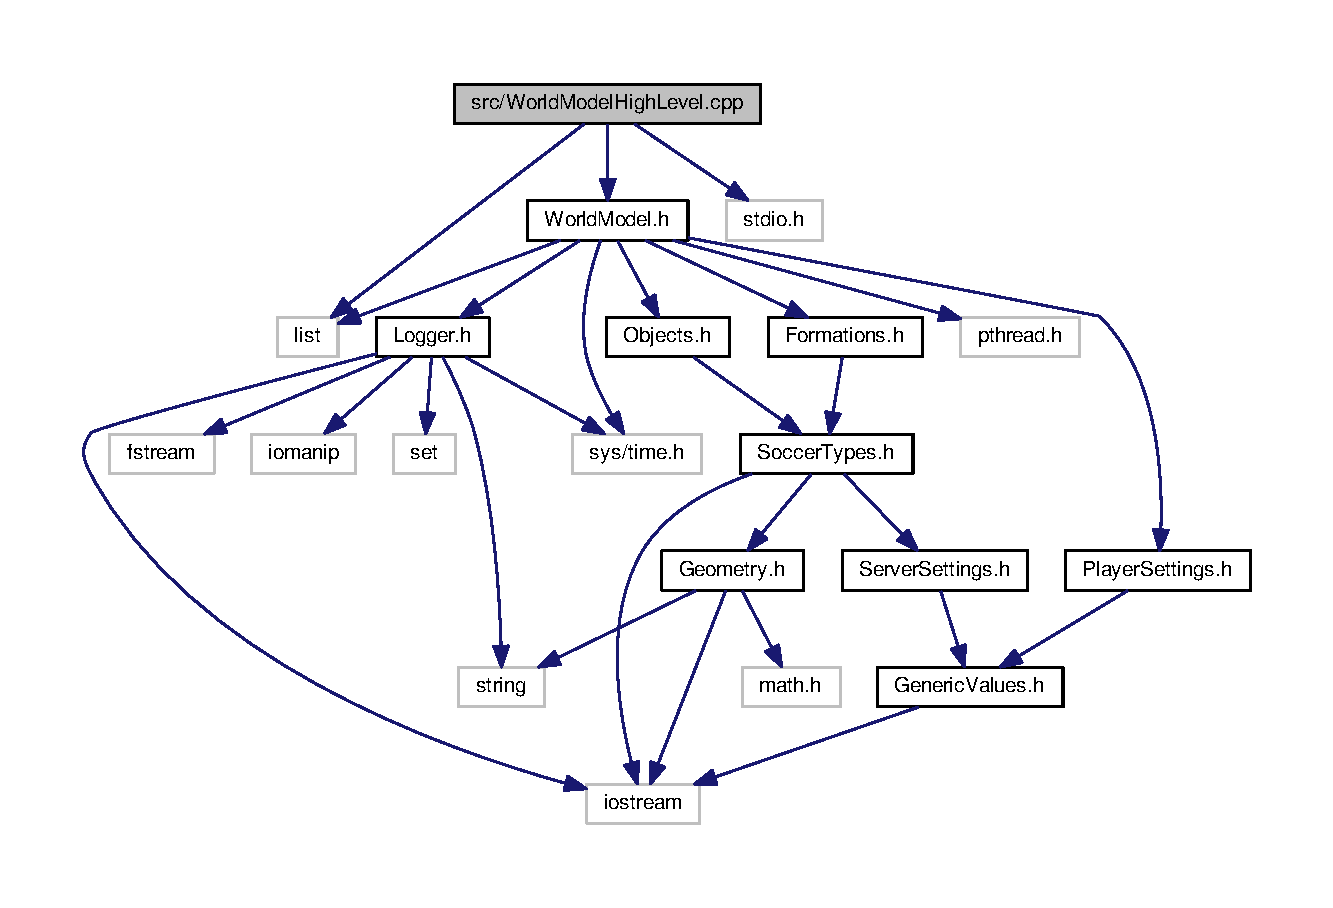
\includegraphics[width=350pt]{WorldModelHighLevel_8cpp__incl}
\end{center}
\end{figure}


\subsection{Detailed Description}

\begin{DoxyPre}
{\bfseries File:}          \hyperlink{WorldModelHighLevel_8cpp}{WorldModelHighLevel.cpp}
{\bfseries Project:}       Robocup Soccer Simulation Team: UvA Trilearn
{\bfseries Authors:}       Jelle Kok
{\bfseries Created:}       12/02/2001
{\bfseries Last Revision:} $ID\$
{\bfseries Contents:}      class definitions of \hyperlink{classWorldModel}{WorldModel}. This class contains
               methods that reason about the world model on a higher
               level and return more abstract information about the current
               world state.



\subsubsection*{{\bfseries Changes}}\end{DoxyPre}



\begin{DoxyPre}
{\bfseries Date}             {\bfseries Author}          {\bfseries Comment}
12/02/2001       Jelle Kok       Initial version created
\end{DoxyPre}
 